\documentclass[12pt]{article}

\usepackage[margin=1in]{geometry}		% For setting margins
\usepackage{amsmath}
\usepackage{graphics}% For Math
\usepackage{fancyhdr}				% For fancy header/footer
\usepackage{graphicx}				% For including figure/image
\usepackage{cancel}				% To use the slash to cancel out stuff in work
\usepackage[english]{babel}
\usepackage{hyperref}
\usepackage{amsfonts}
\usepackage{amssymb}
\documentclass{article}
\usepackage{float}

%%%%%%%%%%%%%%%%%%%%%%
% Set up fancy header/footer
\pagestyle{fancy}
\fancyhead[LO,L]{DATA SCIENCE I}
\fancyhead[CO,C]{FINESI}
\fancyhead[RO,R]{\today}
\fancyfoot[LO,L]{}
\fancyfoot[CO,C]{\thepage}
\fancyfoot[RO,R]{}
\renewcommand{\headrulewidth}{0.4pt}
\renewcommand{\footrulewidth}{0.4pt}
%%%%%%%%%%%%%%%%%%%%%%

\begin{document}

\noindent \textbf{National University of the Altiplano\\
Faculty of Statistical Engineering and Computer Science\\
Theacher: } Fred Torres Cruz\\
\textbf{Author :} Roberth Carlos GONZALES MAURICIO.\\


\noindent
\textbf{ Acceso a crédito de pequeños y medianos productores agropecuarios del Perú: a quién priorizar y qué acciones impulsar (ENA 2016--2025)}

\renewcommand{\figurename}{Figura}
\renewcommand{\tablename}{Tabla}
\renewcommand{\refname}{Referencias}

\section{Objetivo}
Identificar a qué productores conviene dirigir primero la oferta de crédito agropecuario y qué acciones elevarían más su acceso, a partir de un modelo de clasificación construido en R con la Encuesta Nacional Agropecuaria (ENA). La variable objetivo es \texttt{ACCESO\_CREDITO} (1 = obtuvo crédito, 0 = no obtuvo).

\section{Datos y método}
\textbf{Datos.} 49\,837 productores de la ENA 2016, 2017, 2019 y 2022--2025: 39\,868 para entrenar y 9\,969 para probar, separados por conglomerado para que ningún vecindario aparezca en ambos grupos. Solo el 11.9\,\% obtuvo crédito (Costa 20.4\,\%, Selva 12.7\,\%, Sierra 7.5\,\%, con ponderación muestral).

\textbf{Selección de variables.} De 35 candidatas se eligieron 14 en tres pasos: importancia SHAP en validación cruzada, eliminación de variables redundantes (correlación de Spearman $\geq 0.70$) y regla de un error estándar para quedarse con el modelo más simple.

\textbf{Modelo.} XGBoost entrenado con \texttt{caret}: 40 combinaciones de hiperparámetros evaluadas con validación cruzada de 5 pliegues agrupada por conglomerado y elegidas por AUC-PR. Como contraste se ajustó una regresión logística analizada con \texttt{easystats}. Los efectos se interpretaron con \texttt{shapviz}.

\textbf{Análisis prescriptivo.} Con el modelo final se hicieron tres ejercicios sobre el conjunto de prueba: (1) \textit{focalización}, ordenando a los productores por su probabilidad de crédito; (2) \textit{escenarios}, cambiando una condición solo en quienes no la tienen y recalculando la probabilidad; y (3) \textit{demanda potencial}, ubicando a los productores sin crédito cuyo perfil es igual al de quienes sí lo tienen.

\section{Qué tan confiable es el modelo}
En la prueba el modelo alcanza AUC-ROC 0.798, AUC-PR 0.367 (el azar daría 0.119) y MCC 0.307; la regresión logística llega a 0.791, 0.359 y 0.308. Las probabilidades están bien calibradas: al 10\,\% con mayor puntaje se le predice 42.0\,\% y el valor real es 42.7\,\%. El desempeño es estable por año (AUC-ROC de 0.754 a 0.827) y por región (0.761 a 0.787). Esto permite usar las probabilidades para ordenar y simular.

Los factores que más pesan son la superficie cosechada, la edad, el departamento, el tamaño del hogar y el uso de fertilizantes (Figura \ref{fig:shap}). La logística confirma el sentido de los efectos: estar asociado duplica la posibilidad de crédito (\textit{odds ratio} 2.12; IC 95\,\%: 1.92--2.34), arrendar tierra la multiplica por 1.51 y cada 10 años de edad la reducen 17\,\%.

\begin{figure}[!htb]
\centering
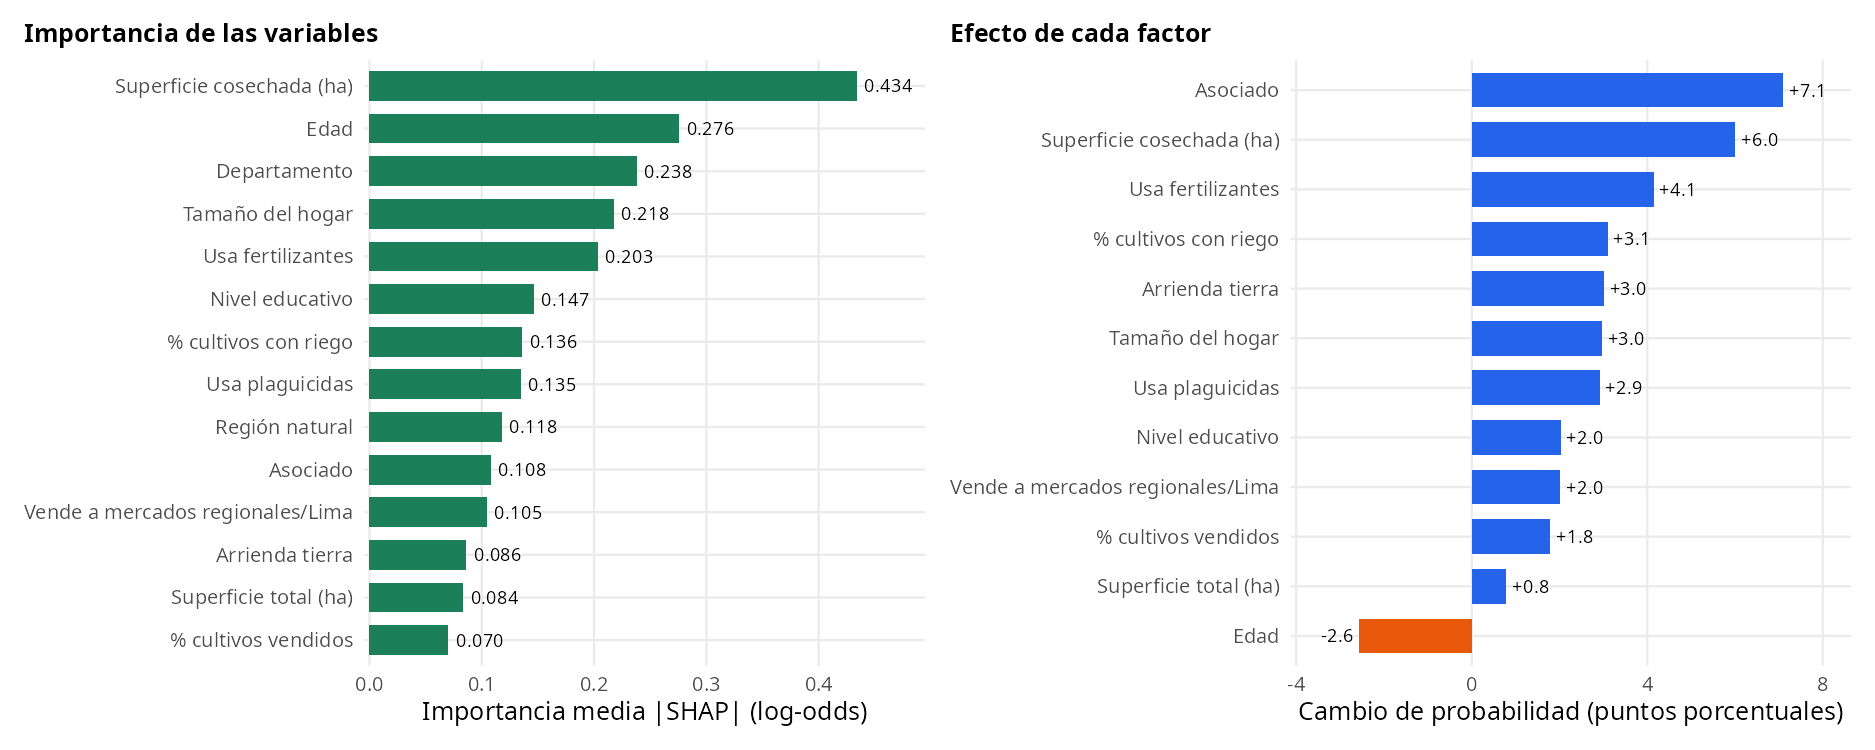
\includegraphics[width=0.95\textwidth]{figuras/06_importancia_efectos.png}
\caption{Importancia de las 14 variables y cambio de la probabilidad de crédito asociado a cada factor.}
\label{fig:shap}
\end{figure}

\section{Análisis prescriptivo}
\subsection{A quién priorizar}
Si se ordena a los productores por la probabilidad que da el modelo, atender al 10\,\% superior alcanza al 36\,\% de quienes obtienen crédito; con el 20\,\% se llega al 54\,\% y con el 30\,\% al 67\,\% (Figura \ref{fig:presc}, izquierda). En el primer tramo, 43 de cada 100 productores obtienen crédito, 3.6 veces más que en una selección al azar.

\subsection{Demanda potencial sin atender}
El 16.4\,\% de los productores (1\,636 de 9\,969) no tiene crédito pero su perfil es igual al de quienes sí lo tienen. Es el grupo donde una oferta de crédito tendría mejor respuesta (Tabla \ref{tab:perfil}): cosechan más de 3 hectáreas, casi todos usan fertilizantes y la mitad ya vende a mercados regionales. Se concentran en Tumbes (45\,\% de sus productores), Tacna (36\,\%), Lambayeque (33\,\%), Ica (27\,\%) y Madre de Dios (26\,\%).

\begin{table}[!htb]
\centering
\caption{Perfil de los productores con crédito, de la demanda potencial y del resto sin crédito}
\label{tab:perfil}
\begin{tabular}{lrrr}
\hline
Característica & Con crédito & Potencial & Resto \\
\hline
Productores & 1\,187 & 1\,636 & 7\,146 \\
Hectáreas cosechadas (mediana) & 2.50 & 3.16 & 0.55 \\
Edad promedio (años) & 50.4 & 50.4 & 56.3 \\
Asociados (\%) & 15.1 & 19.6 & 2.7 \\
Usan fertilizantes (\%) & 79.8 & 88.1 & 47.2 \\
Venden a mercados regionales (\%) & 50.5 & 53.9 & 18.0 \\
Cultivos con riego (\%) & 59.5 & 61.8 & 38.0 \\
Viven en la Sierra (\%) & 39.3 & 30.7 & 66.7 \\
\hline
\end{tabular}
\end{table}

\subsection{Qué acciones elevan más el acceso}
La Figura \ref{fig:presc} (derecha) muestra cuánto subiría la tasa de crédito de cada región si los productores que hoy no tienen una condición la tuvieran. A nivel nacional la tasa estimada es 12.3\,\%:
\begin{itemize}
\item \textbf{Asociatividad}: subiría a 18.7\,\% (+6.4 puntos). Es la acción de mayor efecto en las tres regiones y el 93\,\% de los productores aún no está asociado.
\item \textbf{Riego}: +1.5 puntos en el país, pero +3.6 en la Selva, donde el 97\,\% no riega todos sus cultivos.
\item \textbf{Venta a mercados regionales o Lima}: +1.2 puntos; el mayor efecto está en la Sierra (+1.3), donde el 81\,\% no accede a esos mercados.
\item \textbf{Uso de fertilizantes}: +1.2 puntos; +2.3 en la Selva.
\item \textbf{Acciones combinadas}: asociatividad más mercado sube la tasa a 20.3\,\% (+8.0); las cuatro juntas a 25.1\,\% (+12.8), y en la Selva de 13.1\,\% a 32.3\,\%.
\end{itemize}

\begin{figure}[!htb]
\centering
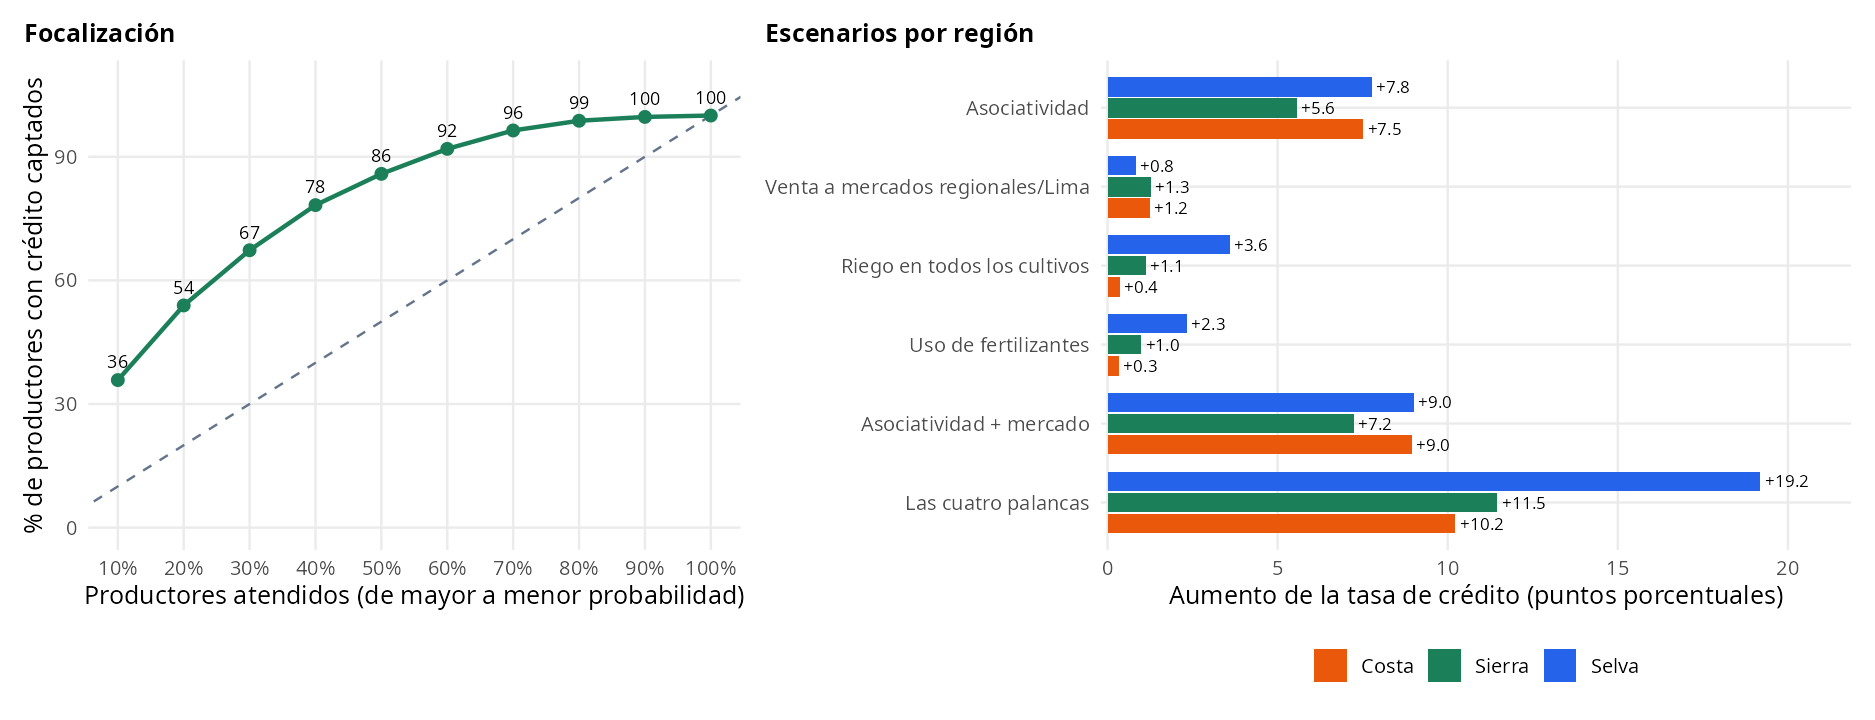
\includegraphics[width=\textwidth]{figuras/08_prescripcion.png}
\caption{Focalización (porcentaje de productores con crédito captados según la cobertura) y aumento simulado de la tasa de crédito por acción y región.}
\label{fig:presc}
\end{figure}

\section{Líneas de acción}
\begin{enumerate}
\item \textbf{Focalizar con el modelo.} Dirigir la promoción de crédito al 20\,\% de productores con mayor probabilidad: ahí está más de la mitad de la demanda efectiva.
\item \textbf{Atender primero la demanda potencial.} Ofrecer crédito a los productores sin crédito con perfil de acreditado, empezando por Tumbes, Tacna, Lambayeque, Ica y Madre de Dios. No requieren cambiar su forma de producir, solo que la oferta llegue.
\item \textbf{Promover la asociatividad.} Es la acción con mayor retorno en todas las regiones; conviene vincular el crédito a cooperativas y asociaciones de productores.
\item \textbf{Diferenciar por región.} Selva: riego y uso de insumos junto con asociatividad. Sierra: asociatividad y articulación a mercados regionales. Costa: asociatividad, porque riego e insumos ya están extendidos.
\item \textbf{Diseñar productos para quienes quedan fuera.} El 72\,\% restante cosecha media hectárea y tiene 56 años en promedio; el crédito convencional no le llega. Se requieren microcréditos, garantías grupales y asistencia técnica previa. Áncash, Loreto, Huánuco y Huancavelica necesitan primero ampliar la oferta financiera.
\end{enumerate}

\section{Limitaciones}
Los escenarios son estimaciones del modelo, no experimentos: indican asociación, no causa segura (un productor puede usar fertilizantes porque ya obtuvo crédito), por lo que conviene validarlos con programas piloto. La precisión del modelo es 0.30, suficiente para priorizar grupos pero no para decidir caso por caso. No se incluyen 2014, 2015, 2018, 2020 ni 2021 por falta de variables o de encuesta.

\section{Conclusiones}
\begin{enumerate}
\item El modelo ordena bien a los productores: el 20\,\% superior concentra el 54\,\% del crédito.
\item Existe una demanda potencial sin atender de 16.4\,\% de los productores, ubicada sobre todo en la Costa.
\item La asociatividad es la acción de mayor impacto (+6.4 puntos); combinada con mercado, riego e insumos duplicaría la tasa de acceso (de 12.3\,\% a 25.1\,\%).
\item Las acciones deben diferenciarse por región y complementarse con productos financieros para los productores más pequeños.
\end{enumerate}

\end{document}
